\section{Introduction}

The flow past bluff bodies and the formation of vortex structures in their wake has attracted the attention of many scholar over the last decades, as they are ubiquitous in natural environments and in several engineering applications \citep{oertel-1990,williamson-1996b,choi-etal-2008,thompson-etal-2021}. Two-dimensional and symmetric bluff bodies isolated in free stream are the prototype of this kind of flows.

Most studies on 2D bluff bodies have focused on the circular and square cylinders to characterise the flow bifurcations. The low-$Re$ steady flow generally becomes unstable to oscillatory perturbations that lead to the von K\'{a}rm\'{a}n vortex shedding. The wake past a circular cylinder, for example, undergoes a Hopf bifurcation at a Reynolds number of $Re = U_\infty D /\nu = 47$, where $U_\infty$ is the free stream velocity and $D$ is the radius of the cylinder \cite{noack.eckelmann-1994-globalstability}. This first Hopf bifurcation is generic to flows past isolated 2D bodies that respect the top/down reflectional symmetry \citep{jackson-1987-finiteelementstudy,chiarini-quadrio-auteri-2022b}. The triggering mechanism of this bifurcation is known to result from a global instability \citep{jackson-1987-finiteelementstudy}, which arises when the region of local absolute instability is large enough \citep{chomaz-2005}. Accordingly, \cite{chiarini-quadrio-auteri-2022b} observed that the onset of this instability depends on the size of the wake recirculating region and on the maximum reverse flow velocity.
%
The secondary instability of the wake past 2D symmetric bluff bodies is generally thought to lead to a three-dimensional flow. For the circular cylinder, for example, the periodic von K\'{a}rm\'{a}n wake undergoes a secondary pitchfork bifurcation at $Re \approx 190$: the flow becomes three-dimensional but retains the same periodicity. \cite{barkley-henderson-1996} found by Floquet stability analysis that the two-dimensional von K\'{a}rm\'{a}n wake becomes unstable to the synchronous three-dimensional mode $A$ which has spanwise wavelength $\lambda \approx 3.9 D$ at $Re \approx 190$, and to mode $B$ with $\lambda \approx 1.2 D$ at slightly larger $Re$. The following studies of \cite{henderson-barkley-1996} and \cite{henderson-1997} showed that the onset of modes $A$ and $B$ are due to a supercritical and subcritical bifurcation, respectively. A quasi-periodic mode $S$ with $\lambda \approx 2.5D$ has been also found to become unstable at larger $Re$ \citep{blackburn-lopez-2003,blackburn-etal-2005,blackburn-sheard-2010}. 
%
\cite{ryan-thompson-hourigan-2005} investigated the secondary instability of the flow past streamlined elongated cylinders (the flow does not separate at the LE in these cases), and found that the secondary bifurcation leads to a 3D flow for all cases. However, they found that the most unstable mode, and therefore the sequence of bifurcations the flow unergoes, changes with the aspect ratio $\AR=L/D$ of the body. They found mode $A$ and two new modes, called mode $B'$ and $S'$ in analogy with the circular cylinder case. Mode $B'$ possesses the same spatio-temporal symmetry as mode $B$, but a spanwise wavelength and near-wake features that are more similar to mode $S$. Mode $S'$ is time-varying from one shedding period to the next one, similarly to mode $S$ for the square and circular cylinder \citep{robichaux-balachandar-vanka-1999}, but exhibits a perturbation field that is reminiscent of mode $B$. \cite{ryan-thompson-hourigan-2005} observed that for small aspect ratios, i.e. $\AR \le 7.5$, the first mode to become unstable is mode $A$, while for larger $\AR$ the first mode to become unstable is $B'$. 

We now move to two-dimensional symmetric bluff bodies with sharp LE corners, that are the focus of the present work. Unlike circular and streamlines cylinders, in this case the presence of the corners at the LE enforces the flow separation. The flow past rectangular cylinders with blunt LE is the prototype of this kind of flows, and has been largely investigated over the last years at both (relatively) low \citep{hourigan-thompson-tan-2001,zhang-etal-2023} and large \citep{cimarelli-leonforte-angeli-2018,chiarini-etal-2022,cimarelli-etal-2024} Reynolds numbers. Varying the aspect ratio a wide range of bodies is obtained, from a flat plate placed normal to the incoming flow for $\AR \rightarrow 0$, to a flat plate parallel to the incoming flow for $\AR \rightarrow \infty$. Notably, already at intermediate Reynolds numbers after the primary Hopf bifurcaton, i.e. $Re \approx 200-400$, the flow physics is extremely rich and largely depends on $\AR$ \citep[see for example][]{okajima-1982,nakamura-etal-1991,mills-etal-1995}. For $\AR \le 1$ the shear layers that separate at the LE roll up in the wake and create the classical von K\'{a}rm\'{a}n vortex street; in this case the flow dynamics resembles that of the circular cylinder case. For intermediate aspect ratios, i.e. $1 \le \AR \le 3$, the shear layers separating from the LE reattach intermittently over the lateral sides of the cylinder: a recirculating region intermittently arises there. For larger $\AR$, instead, the LE shear layers reattach along the top/bottom lateral sides of the cylinder permanently, and generate large recirculating regions that periodically enlarge and shrink. At large enough $Re$, for these larger $\AR$ vortex shedding occurs from both the LE and TE shear layers and the two phenomena lock to the same frequency due to the so-called ILEV instability, leading to an almost stepwise dependence of the Strouhal number $St_L=fL/U_\infty$ on $\AR$ \citep{okajima-1982,nakamura-etal-1991,hourigan-thompson-tan-2001}; see figure \ref{fig:StLAR}. 
%
\begin{figure}
  \centering
   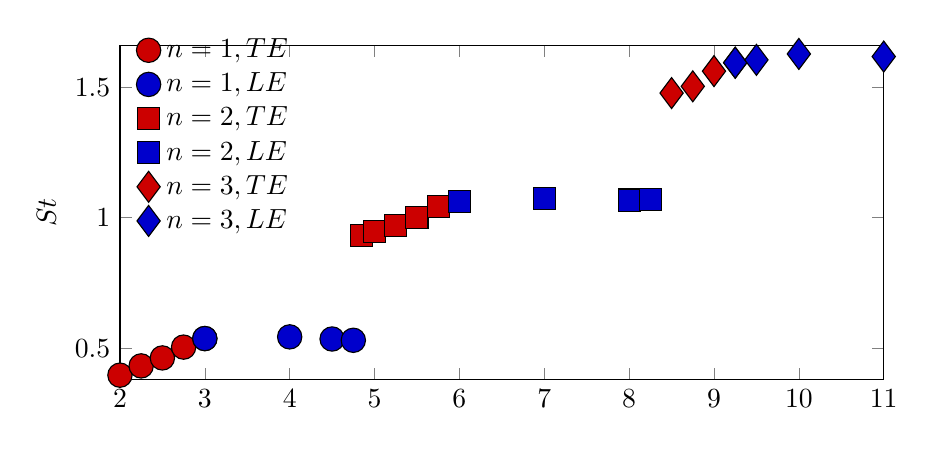
\begin{tikzpicture}



\begin{axis}[%
%width=4.3cm,
%height=3.5cm,
width=0.8\textwidth,
height=0.35\textwidth,
scale only axis,
%grid=both,
%axis lines=middle,
xmin=2,
xmax=11,
ymin=0.38,
ymax=1.66,
%xtick={2, 3, 4, 5, 6, 7, 8, 9, 10, 11},
%ytick={0.4, 0.6, 0.8, 1, 1.2, 1.4, 1.6, 1.8},
%xlabel style={font=\color{white!15!black}},
xlabel={\AR},
ylabel={$St$},
%ymin=0,
%ymax=200,
axis background/.style={fill=white},
legend style={at={(0.01,0.73)}, anchor=west, legend cell align=left, align=left, fill=none, draw=none}
]

\addplot [color=black,only marks,mark=*,mark options={scale=2.2,black,fill=red!80!black}]
  table[row sep=crcr]{%
2       0.396741726829078\\
2.25    0.432248406188668\\
2.5     0.462793383468913\\
2.75    0.504214143890634\\
3       0.536994008053543\\
};
\addlegendentry{$n=1,TE$}

\addplot [color=black,only marks,mark=*,mark options={scale=2.2,black,fill=blue!80!black}]
  table[row sep=crcr]{%
3       0.536994008053543\\
4       0.543439544221324\\
4.5     0.535298051494477\\
4.75    0.530324957725253\\
};
\addlegendentry{$n=1,LE$}


\addplot [color=black,only marks,mark=square*,mark options={scale=2,black,fill=red!80!black}]
  table[row sep=crcr]{%
4.85    0.930407996044941\\
5       0.947349623285183\\
5.25    0.971304878725648\\
5.5     1.000378564453700\\
5.75    1.041747167637721\\
6       1.062464533558995\\
};
\addlegendentry{$n=2,TE$}

\addplot [color=black,only marks,mark=square*,mark options={scale=2,black,fill=blue!80!black}]
  table[row sep=crcr]{%
6       1.062464533558995\\
7       1.073230579537877\\
8       1.067458930414985\\
8.25    1.070000000000000\\
};
\addlegendentry{$n=2,LE$}


\addplot [color=black,only marks,mark=diamond*,mark options={scale=2.8,black,fill=red!80!black}]
  table[row sep=crcr]{%
8.5     1.477258532919061\\
8.75    1.503123920971757\\
9       1.561211928154617\\
9.25    1.593577708455838\\    
};
\addlegendentry{$n=3,TE$}

\addplot [color=black,only marks,mark=diamond*,mark options={scale=2.8,black,fill=blue!80!black}]
  table[row sep=crcr]{%
9.25    1.593577708455838\\    
9.5     1.604355188881951\\
10      1.627228310690177\\
11      1.617135083478177\\
};
\addlegendentry{$n=3,LE$}



%\addplot [color=black,solid,mark=square*,mark options={scale=0.9,black,fill=red!80!black}]
%  table[row sep=crcr]{%
%3       0.609743754434522\\
%4       0.774727821194389\\
%5       0.942866305443131\\
%6       1.100079139112736\\
%7       1.245663824885169\\
%8       1.400191666484032\\
%9       1.546133959599630\\
%10      1.685632118301302\\
%11      1.822225132985195\\
%};



\end{axis}


\end{tikzpicture}%

   \caption{Dependence of $St_L$ on $\AR$ at $Re=400$. Figure adapted from \cite{chiarini-quadrio-auteri-2022}.}
   \label{fig:StLAR}
\end{figure}
%
This stepwise change of $St_L$ is related to the number $n$ of LE vortices that are simultaneously accommodated along the lateral sides of the cylinder, being for example $n=1$ for $\AR=4$, $n=2$ for $\AR=7$ and $n=3$ for $\AR=9$. \cite{chiarini-quadrio-auteri-2022} observed that two different regimes are possible depending on the relative phase between the LE and TE vortices and on the prevalence of either shedding. When the LE vortices dominate the shedding frequency locks to the passing frequency of the LE over the TE and $St \approx n U_c$, where $n$ is the number of LE vortices present simultaneously over the sides of the cylinder and $U_c \approx 0.55 U_\infty$ is the mean convection velocity of the LE vortices \citep[see also][]{mills-sheridan-hourigan-2002,tan-thompson-hourigan-2004}. In contrast, when the TE vortices dominate the flow matches the frequency of elongated bodies with same $\AR$, but rounded LE that does not produce flow separation. Using dynamic mode decomposition, \cite{zhang-etal-2023} observed that the feedback mechanism at $Re = 1000$ changes with $\AR$. For small $\AR$, the feedback loop encompasses the whole separation region and the flow is controlled by the impinging shear-layer instability; for larger $\AR$, the feedback loop covers the entire chord of the cylinder and the flow is controlled by the leading-edge vortex shedding instability.
  
The presence of different regimes and LE/TE vortex interactions hints for the existence of different secondary instabilities and thus different routes to turbulence. To the best of our knowledge, however, a complete picture is still missing and little is known about the secondary instability of the flow past elongated rectangular cylinders with $\AR>1$. It is well established that the flow past a square cylinder ($\AR=1$) undergoes the same sequence of bifurcations mentioned for the circular cylinder case, albeit the primary and secondary instabilities occur at a slightly lower Reynolds number \citep[see for example][]{jiang-cheng-2018,blackburn-sheard-2010}. Indeed, \cite{robichaux-balachandar-vanka-1999}, \cite{blackburn-lopez-2003}, \cite{sheard-fitzgerald-ryan-2009}, \cite{blackburn-sheard-2010} found via Floquet stability analysis that the flow becomes $3D$ due to mode $A$ at $Re \approx 165$, and that modes $B$ and $S$ become unstable only at larger $Re$. By means of 3D Direct Numerical Simulations (DNS), \cite{sheard-fitzgerald-ryan-2009} and \cite{jiang-cheng-an-2018} discussed the saturation effect of the nonlinear terms on the growth of the different modes. \cite{sheard-fitzgerald-ryan-2009} found that the appearance of both modes $A$ and $B$ is due to a supercritical bifurcation. However, \cite{jiang-cheng-an-2018} remarked that, unlike the circular cylinder case \citep{henderson-1997}, the instability of mode A is subcritical; they explained the discrepancy with the results of \cite{sheard-fitzgerald-ryan-2009} with the small computational domain adopted in the latter study. \cite{sheard-fitzgerald-ryan-2009} and \cite{sheard-2011} studied how the angle of incidence affects the unstable modes: mode $A$ is the most unstable one at small and large incidences, while a subharmonic mode, called $C$, is the most unstable at intermediate angles. \cite{choi-yang-2014} considered the flow past rectangular cylinder with $\AR \le 1$, ranging from a flat plate normal to the flow ($\AR \rightarrow 0$) to a square cylinder ($\AR=1$). They found that when reducing $\AR$ both modes $A$ and $B$ stabilise and that new modes A2 and QP2 of synchronous and quasi periodic nature become unstable \citep[see also][]{thompson-etal-2006}. \cite{chaurasia-thompson-2011} and \cite{huang-etal-2017} studied the flow past a semi-indefinite plate of finite thickness, i.e. a rectangular cylinder with $\AR \rightarrow \infty$. The found that the vortices that arise from the LE shear layer due to an induced Kelvin--Helmholtz instability become unstable to subharmonic 3D perturbations at $Re \approx 380$. Despite these works, however, almost no information is available for the secondary bifurcation of the flow past elongated rectangular cylinders with $1 < \AR < \infty$. In a recent work \citep{chiarini-quadrio-auteri-2022d}, we have considered the specific $\AR=5$ ($n=2$ regime dominated by the TE vortex shedding) that defines the BARC benchmark, and found that the secondary instability is due to the QS mode which is of quasi subharmonic nature. Specifically, we found that the wavemaker \citep{monkewitz-huerre-chomaz-1993} of this instability is localised in the region over the longitudinal sides of the cylinder, and that the instability is triggered by the mutual inviscid interaction of the vortices generated by the LE shear layer. It is thus clear that a complete characterisation of how the different flow regimes and LE/TE vortex interaction influence the secondary instability of the flow past rectangular cylinder with $\AR>1$ and thus its route to turbulence is lacking.
    
The aim of this work is to do a step forward in this direction. We aim to fill the gap and characterise the secondary bifurcation of the flow past rectangular cylinders with $1 \le \AR \le 9$ by means of both stability analysis and fully nonlinear 3D DNS. In this work, besides characterising how the different LE/TE vortex interactions influence the bifurcation scenario, we will also provide insights on the triggering mechanism of mode $A$. As shown in the following, indeed, mode $A$ is found only in the regimes dominated by the TE vortices. 
  
The remainder of the work is structured as follows ...
